\subsection{ВЭПП-2000}

Сканирующий ускорительный комплекс со встречными элек\-т\-рон-по\-зи\-т\-рон\-ны\-ми пучками ВЭПП-2000 в ИЯФ СО РАН работает с 2010 года в диапазоне энергий в системе центра масс пучков от \SI{320}{\MeVr} до \SI{2007}{\MeVr} \cite{Berkaev2012}.

Коллайдер использует одно кольцо и рабоатет в режиме сгусток--сгусток
с использованием круглых пучков \cite{Danilov:1996jw}.
Фокусировка в месте встречи осуществляется с помощью сверхпроводящих магнитов с полем \SI{13}{\teslaru}.

\begin{figure}[htbp]
    \centering
    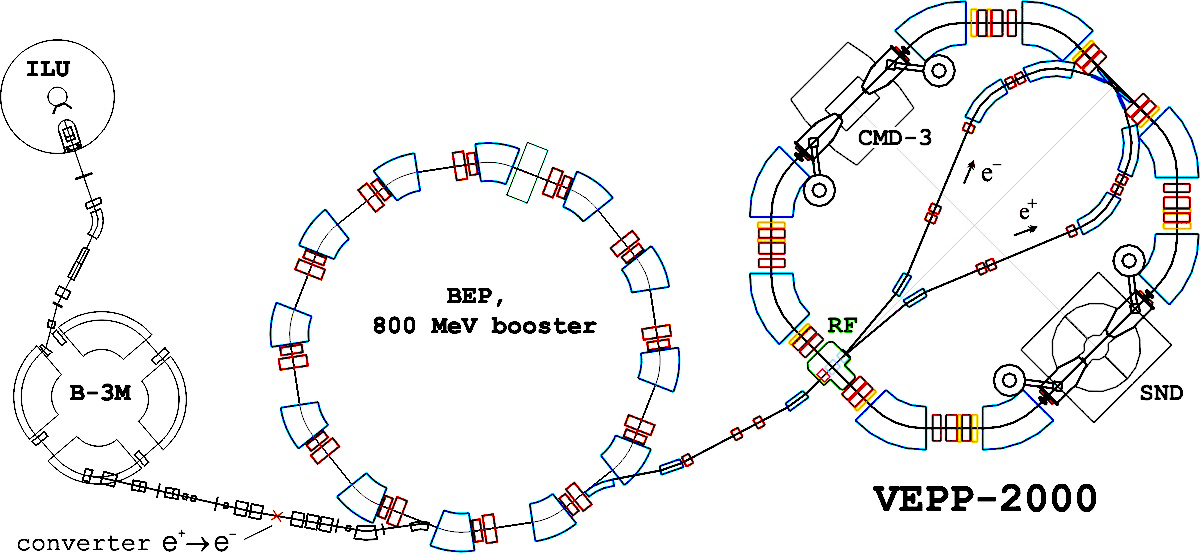
\includegraphics[width=\textwidth]{img/vepp2knew.png}
    \caption{Схема ускорительного комплекса ВЭПП-2000 до 2014 года.}
    \label{fig:vepp2000}
\end{figure}

Схема ускорительного комплекса до 2013 года представлена на Рис.~f\ref{fig:vepp2000}.
Комплекс состоял из импульсного линейного ускорителя ИЛУ,
синхротрон Б3-М,
конвертора,
бустурного кольца БЭП
и коллайдера ВЭПП-2000.

В 2013--2016 годах была проведена модернизация комлекса.
главным образом направленая на использования нового инжекционного комплекса ВЭПП-5
и улучшение БЭП,
позволяющие теперь ускорять и инжектировать пучки на энергии эксперимента,
то есть до \SI{1}{\GeVr}.

В 2017 году была возобновлена работа ускорительного комплекса и достигнуты значения светимости
\SI{3e31}{\cmr^{-2} \sr^{-1}} на энергии $\sqrt{s} = \SI{2}{\GeVr}0$ \cite{Shatunov:2018xfm}.

В местах встречи пучков на коллайдере установлено и работает два универсальных детектора КМД-3 и СНД.





\subsubsection{Измерение энергии пучков}

Для измерения энергии пучков на коллайдере ВЭПП-2000 используется метод с обратным комптоновским рассеянием монохроматичных фотонов \ce{CO}-лазера на электронном пучке, \cite{laserBeamAbakumova2014}.
Что позволяет измерять энергию пучков с относительной систематической ошибкой порядка \num{6e-5}.


% Для проверки корректности работы лазера и для определения энергии для статистики,
% набранной раньше установки и введения в работу лазера,
% используются измерения полной энергии системы с помощию процессов с присутствием заряженных частиц в конечном состоянии.

% Для определения энергии пучков по данным физических процессов используется измерение импульса заряженных частиц в дрейфовой камере.
% Заряженные каоны и пионы, а также протоны можно идентифицировать по удельному энерговыделению $dE/dx$ в дрейфовой камере и по выделившейся энергии в калориметре.
% Так как идентификация частиц основана разделении по $dE/dx$, то надо учитывать его зависимость от импульса частица.
% Также трек частицы в ДК должен иметь достаточно большую кривизну, для корректного определения импульса.
% В следствии этих причин, а также наличия порога реакций, лежащих в области сканирования ВЭПП-2000, для каждого процесса есть область применимости для определения энергии $e^+e^-$--пучков.
% Таким образом:
% \begin{itemize}
%   \item $e^+ e^- \to e^+ e^-$ используется в диапозоне $ \SI{}{\MeVr} < \sqrt{s} < \SI{}{\MeVr} $
%   \item $e^+ e^- \to K^+ K^-$ используется в диапозоне $ \SI{}{\MeVr} < \sqrt{s} < \SI{}{\MeVr} $
%   \item $e^+ e^- \to K^+ K^- \pi^+ \pi^-$ используется в диапозоне $ \SI{}{\MeVr} < \sqrt{s} < \SI{}{\MeVr} $
%   \item $e^+ e^- \to p \bar{p}$ используется в диапозоне $ \SI{}{\MeVr} < \sqrt{s} < \SI{}{\MeVr} $
% \end{itemize}